\section{Zielsetzung}
    Ziel dieses Versuches ist es die Absorption von $\symup{\gamma}$- und $\symup{\beta}$- Strahlung zu messen. Dadurch werden die 
    Absorptionskoeffizienten verschiedener Materialien und die Maximalenergie des $\symup{\beta}$ - Strahlers bestimmt.


\section{Theorie}
\label{sec:Theorie}
Zur Beschreibung der Wechselwirkung von Teilchenstrahlen mit Materie wird ein Wirkungsquerschnitt $\sigma$ definiert. Dieser steht dabei allerdings in 
keinem Zusammenhang zu einem geometrischen Querschnitt, sondern gibt an, wie Strahlung mit einem Absorbermaterial wechselwirkt. Das heißt, bei größerer
Wahrscheinlichkeit der Wechselwirkung ist der Wirkungsquerschnitt ebenfalls größer.
Über den Wirkungsquerschnitt
lässt sich die Anzahl der Wechselwirkungen (für $\gamma$ - Strahler) in einem Absorber zu 
\begin{equation}
    \label{eqn:absorp}
    N(D) = N_0 \cdot e^{-n \sigma D}
\end{equation}
bestimmen, wobei $D$ die Dicke des Absorbers, $n$ die Anzahl der Teilchen pro Volumen und $N_0$ die Ausgangsaktivität ist.
Daraus kann ein Absorptionskoeffizient $\mu$ zu 
\begin{equation}
    \label{eqn:mu}
    \mu = n \sigma
\end{equation}
Die Anzahl der 
Teilchen pro Volumen lässt sich zudem zu 
\begin{equation}
    \label{eqn:anzahl_teilchen}
        n = \frac{z N_{\symup{A}}}{V_{\symup{Mol}}} = \frac{z N_{\symup{A}} \rho}{M}
\end{equation}
bestimmen. Hierbei ist $N_{\symup{A}}$ die Avogardokonstante, $z$ die Ordnungszahl, $V_{\symup{Mol}}$ das Molvolumen, $\rho$ die Dichte und $M$
das Molekulargewicht.
Der Wirkungsquerschnitt $\sigma$ lässt sich dadurch über 
\begin{equation}
    \label{eqn:wirkungsquerschnitt}
    \sigma = \frac{\mu}{n}
\end{equation}
bestimmen. Das hier beschriebene Absorptionsgesetz gilt allerdings nur für die Absorption von $\gamma$ - Strahlung und nur für kleine Dicken $D$ des
Absorbermaterials für $\beta$ - Strahlung.
\subsection{Gamma - Strahlung}
Zur Enstehung von $\gamma$ - Strahlung muss ein angeregter Atomkern auf ein niedrigereres Energienivieau fallen. Die dabei frei werdende 
Energie wird in Form von Photonen emittiert und hat daher Lichtgeschwindigkeit. Gemäß der Quantentheorie sind die Energienivieaus diskrete
Zustände, weshalb auch das Linienspektrum der Strahlung diskret verteilt ist. Des Weiteren weist $\gamma$ - Strahlung auch einige elektromagnetische 
Effekte in Wechselwrikung mit Materie auf.Im Wesentlichen treten drei verschiedene Arten von Wechselwirkunng auf: Annihilation, inelastische 
Streuung und elastische Streuung, wobei sich diese drei Vorgangänge je nach Wechselwirkungspartner nochmals unterscheiden. Eine Übersicht der
möglichen Wechselwirkungen ist in \autoref{fig:tabelle} zu sehen. Am wichtigsten der dargestellten Prozesse sind allerdings der Photo-Effekt,
der Compton-Effekt, sowie die Paarbildung. 
\begin{figure}
        \centering
        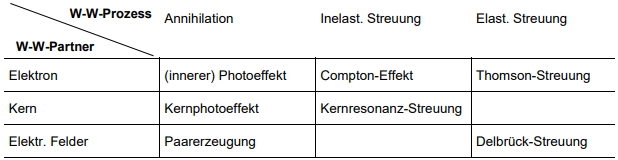
\includegraphics[width=\textwidth]{content/tabelle.png}
        \caption{Die verschiedenen Wechselwirkungen von $\gamma$ Strahlung mit Materue \cite[233]{V704}.}
        \label{fig:tabelle}
    \end{figure}

Beim Photoeffekt löst das einfallende $\gamma$ - Quant ein Elektron aus der Atomhülle. Dabei wird das Quant vernichtet. Das herausgelöste
Elektron erhält die Engergie des Quants, abzüglich der vorher zu überwindenden Bindungsenergie. Daraus folgt auch, dass das einfallende 
Quant eine Energie haben muss, welche größer als die Bindungsenergie ist, da der Photoeffekt sonst nicht stattfinden kann.
Zu Erwähnen sei hierbei noch, dass durch herauslösen eines Elektrons aus einer Schale, ein Elektron einer höheren Schale, unter Aussendung eines
Röntgenquantes, die enstandene Lücke wieder aufgefüllt werden kann.

Der Comptoneffekt tritt bei der Wechselwirkung mit freien Elektronen auf, wie beispielsweise in einem Metall. Hierbei stößt das Quant das Elektron lediglich an,
wird aber nicht vernichtet. Es kommt nur zu einer Abnahme der Intensität des Quants, da hier Energie an das Elektron abgegeben wird. Die Bahnen
beider Wechselwikungspartner wird dabei verändert. Der Wirkungsquerschnitt wird nach Klein und Nishina als 
\begin{equation}
    \label{eqn:wirkung_comp}
    \sigma_{\symup{com}} = 2 \pi r_{\symup{e}}^2 \Bigl(\frac{1 + \epsilon}{\epsilon^2} \Bigl( \frac{2(1 + \epsilon)}{1+ 2 \epsilon} - \frac{1}{\epsilon} \ln(1 + 2 \epsilon)  \Bigr ) + \frac{1}{2 \epsilon} \ln(1 + 2 \epsilon)  - \frac{1 + 3 \epsilon}{(1 + 2 \epsilon)^2} \Bigr )
\end{equation}    
angegeben. Hierbei bezeichnet $\epsilon$ das Verhältnis von der Quantenenergie $E_{\symup{\gamma}}$ zur Ruheenergie des Elektrons mit 
\begin{equation}
    \label{eqn:epsilon}
    \epsilon = \frac{E_{\symup{\gamma}}}{m_0 c^2}
\end{equation}    
und $r_{\symup{e}}$ den klassischen Elektronenradius mit $r_{\symup{e}} = 2,82 \cdot 10^{-15}$ m.

Der letzte der behandelten Fälle ist die Paarbildung, bei der das $\gamma$ - Quant annihiliert wird, wobei ein Positron und ein Elektron enstehen.
Dies tritt ein, wenn die Engergie des Qunates mindestens doppelt so groß wie die Ruhemasse eines Elektrons ist, wobei zur tatsächlichen 
Paarbildung auf Grund der Impulserhaltung höhere Energien erforderlich sind. Allgemein lässt sich für den Wirkungsquerschnitt bei diesem
Prozess aber sagen, dass der Zusammenhang zwischen Wirkungsquerschnitt und Ordnungszahl $z$ gegeben ist durch $ \sigma_{\symup{p}} \propto z^2$.

Insgesamt überlagern sich die beschriebenen Effekte beim Durchgang von Materie, wobei die auftretenden Effekte vorallem von der Energie 
des $\gamma$ - Quantes abhängen. Für Germanium ist hierzu ein Diagramm in \autoref{fig:energie} dargestellt. Zu sehen ist, dass bei geringen 
Energien der Photoeffekt überwiegt, worauf bei mittleren Energien der Comptoneffekt folgt und schließlich bei hohen Engergien die Paarbildung 
am meisten stattfindet. Es ist davon auszugehen, dass oberhalb von $100$ MeV nur noch Paarbildung stattfindet. Aus den drei einzelnen Kurven
kann durch Überlagerung die Totalkurve gebildet werden.
\begin{figure}
        \centering
        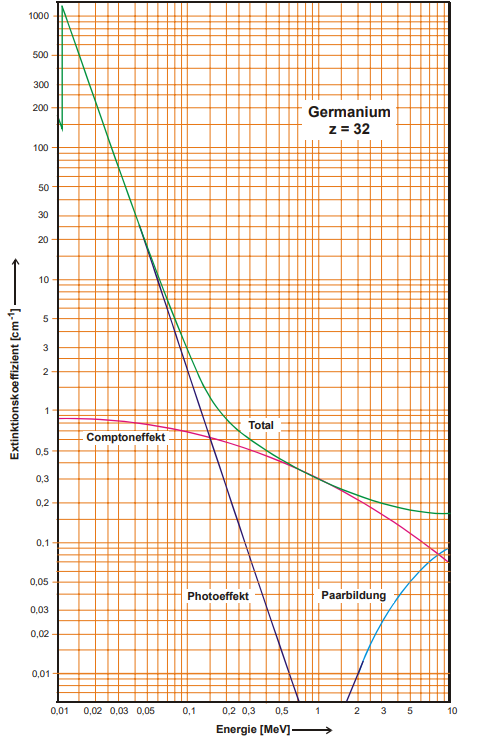
\includegraphics[width=\textwidth]{content/energieabhaengigkeit.png}
        \caption{Energieabhängigkeit des Absorptionskoeffizienten $\mu$ für Germanium, mit den verschiedenen auftretenden Wechselwirkungen und dem Totaleffekt\cite[236]{V704}.}
        \label{fig:energie}
    \end{figure}

\subsection{Beta - Strahlung}
Die $\beta$ - Strahlen sind positiv oder negativ geladene Elektronen, welche bei dem Zerfall eines Protons, beziehungsweise Neutrons enstehen.
Dies geschieht unter der Bildung eines Neutrinos, beziehungsweise Antineutrinos:
\begin{align}
    \label{eqn:kernreaktionen}
    n &\to p + \beta^{-} + \overline{\nu_{\symup{e}}} \\
    p &\to n + \beta^{+} + \nu_{\symup{e}}. 
\end{align}     
Bei diesem Prozess erhält das $\beta$ - Teilchen die gesamte frei werdende Energie, weshalb das Energiespektrum kontinuierlich ist.
Daher entspricht diese Energie auch der Maximalenergie der $\beta$ -Strahlung.
Die $\beta$ - Strahlung kann an Materie streuen, wobei hier drei dieser Streuprozesse näher beleuchtet werden.


Bei der elastischen Streuung am Atomkern, auch bekannt unter dem Namen Rutherford-Streuung, werden die eintreffenden Elektronen 
im Coloumbfeld des Atomkerns gestreut, was zu starken Richtungsänderungen des Elektrons führen kann. Dies bewirkt einerseits, dass sich das
Strahlenbündel auffechert und damit an Intensität verliert und andererseits werden die Bahnlängen der $\beta$ - Teilchen erheblich größer,
als ihre Reichweite $R$, was die Wahrscheinlichkeit erneuter Wechselwirkung deutlich erhöht. Insgesamt ist aber festzuhalten, dass
der Energieverlust bei dieser Streuung als gering einzustufen ist.

Ein weiterer Streueffekt ist die inelastische Streuung an Atomkernen. Hierbei werden die eintreffenden Elektronen im Coloumbfeld des Atomkerns
beschleunigt, was zur Emission von Strahlung führt. Die enstandene Strahlung führt zur Abbremsungs des Elektrons und wird daher als 
Bremsstrahlung beichnet. Der Wirkungsquerschnitt bei diesem Prozess ist gegeben durch
\begin{equation}
    \label{eqn:wirkung_inelastisch}
    \sigma_{\symup{Br}} = \alpha r_{\symup{e}}^2 z^2,
\end{equation}
wobei $\alpha$ die Sommerfelsche Feinstrukturkonstante ist. Auch hier ist allerdings zu bemerken, dass durch die Bremsstrahlung zwar Energie 
verloren geht, sie aber nicht für den Großteil des Energieverlustes verantwortlich ist. 

Der größte Energieverlust tritt nämlich bei der inelastischen Streuung an den Elektronen im Absorbermaterial auf. Hierbei werden die Absorberatome 
ionisiert beziehungsweise angeregt. Ansich verbraucht die Ioniesierung nicht viel Energie, daher ist es möglich, dass ein $\beta$ - Teilchen mehrere
Ioniesierungen hintereinander durchführt. Die Wahrscheinlichkeit, dass eine solche Anregung stattfindet, ist dabei proportional zur Ordnungszahl
$z$ des Absorbermaterials und der Anzahl der Atome pro Volumen im Material.

Wie bereist erwähnt gilt beim $\beta$ - Strahler das Absorptionsgesetz, wie auch beim $\gamma$ - Strahler. Dies gilt aber nur solange, wie die 
Dicken des Absorbermaterials kleiner als die maximale Reichweite der Strahlung $R_{\symup{max}}$ ist. Werden größere Dicken verwendet, 
tritt nut noch Untergrundstrahlung auf, welche aus Bremsstrahlung und Hintergrundstrahlung besteht. Dieser Zusammenhang ist in \autoref{fig:massenbelegung}
zu sehen, wobei sich die Massenbelegung über 
\begin{equation}
    \label{eqn:massenbelegung}
    R = \rho D
\end{equation}
errechnet. 
\begin{figure}
        \centering
        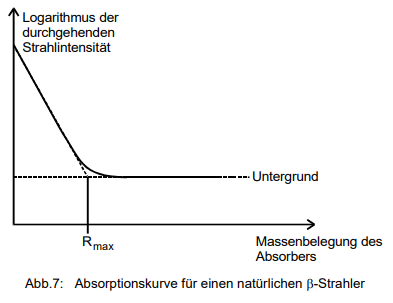
\includegraphics[width=\textwidth]{content/absorption.png}
        \caption{Schematische Absorptionskurve eines $\beta$ - Strahlers\cite[241]{V704}.}
        \label{fig:massenbelegung}
    \end{figure}
Da bei der maximalen Reichweite $R_{\symup{max}}$ vor allem die maximale Energie $E_{\symup{max}}$ auftritt, gilt die empirische Formel:
\begin{equation}
    \label{eqn:max_energie}    
    E_{\symup{max}} = 1,92 \cdot \sqrt{R_{\symup{max}}^2 + 0,22 \cdot R_{\symup{max}}}.
\end{equation}
Hierbei wird $E_{\symup{max}}$ allerdings in $10^6$ eV angegeben.